\documentclass[conference,letterpaper]{IEEEtran}
\IEEEoverridecommandlockouts
% The preceding line is only needed to identify funding in the first footnote. If that is unneeded, please comment it out.
%\usepackage{cite}

\usepackage{mathtext} 		 % русские буквы в формулах
\usepackage[T2A]{fontenc}
\usepackage[utf8]{inputenc}
\usepackage[russian]{babel}

\usepackage{textcomp}

\usepackage{hyphenat}
\hyphenation{ма-те-ма-ти-ка вос-ста-нав-ли-вать}

\usepackage{amsmath,amssymb,amsfonts}
\usepackage{algorithmic}
\usepackage{graphicx}
\usepackage{textcomp}
\usepackage[OT1]{fontenc}
\usepackage{pifont}
\usepackage{multirow}
\usepackage{threeparttable}
\usepackage{booktabs}% http://ctan.org/pkg/booktabs
\newcommand{\tabitem}{~~\llap{\textbullet}~~}

\usepackage{tempora}

%%%%%%%%%%%%%%%%%%%%%%%%%%%%%%%%%%%%%%%%%%
\usepackage[dvipsnames,svgnames]{xcolor, colortbl}
\newcommand{\etal}{{\em et al.\ }}
\newcommand*{\blue}{\textcolor{blue}}
\newcommand*{\red}{\textcolor{red}}
\definecolor{LightCyan}{rgb}{0.88,1,1}
%%%%%%%%%%%%%%%%%%%%%%%%%%%%%%%%%%%%%%%%%%

\usepackage{tikz}
\usetikzlibrary{automata, arrows.meta, positioning}
\usetikzlibrary{graphs,graphs.standard}

\def\BibTeX{{\rm B\kern-.05em{\sc i\kern-.025em b}\kern-.08em
    T\kern-.1667em\lower.7ex\hbox{E}\kern-.125emX}}
\begin{document}
\bstctlcite{IEEEexample:BSTcontrol}

%%----------------------------------------------------------------------------------%%
%% 							TITLE AND LIST OF AUTHOR'S
%%----------------------------------------------------------------------------------%%
\title{Оптимизация условных переходов с учетом векторных возможностей
        потока управления Intel GPU\\
}
%%%---------------- Uncomment for Blind Review -------------------%%
%\author{
%1\textsuperscript{st} Name Surname,
%2\textsuperscript{nd} Name Surname,
%}
%\IEEEauthorblockA{
%\textit{name of organization (of Aff.)}\\
%City, Country \\
%email address}
%}
%%---------------- Uncomment for Blind Review -------------------%%
%%---------------- Uncomment for Final Version -------------------%%
\author{
\IEEEauthorblockN{
Тарасов Юлий Валерьевич,
Владимиров Константин Игоревич
}
\IEEEauthorblockA{
\textit{}\\
\\}
}
%%---------------- Uncomment for Final Version -------------------%%
\maketitle
%%----------------------------------------------------------------------------------%%
%% 									PAPER ABSTRACT
%%----------------------------------------------------------------------------------%%
\begin{abstract}
  Аннотация...
\end{abstract}

%%----------------------------------------------------------------------------------%%
%% 								MAIN CONTENT OF THE PAPER
%%----------------------------------------------------------------------------------%%
\section{Введение}
\label{sec:Introduction}

\section{Аппаратные возможности потока управления}
\label{sec:Goto}

В скалярных архитектурах поток управления обычно реализован через инструкции
условных переходов. При этом условие, от которого зависит переход, всегда также
является скалярным. В отличие от этого в векторной модели может возникать
векторное условие, верное для одних линий исполнения и неверное для других.
В архитектурах не поддерживающих векторный поток управления такой случай может
быть сведен к скалярному путем маскированного исполнения всех инструкций дуги
условного перехода или как минимум маскированного исполнения инструкций этой
дуги, имеющих побочные эффекты (обычно это только записи в память).

В графических ускорителях Intel есть возможность использовать векторный поток
управления без сведения его к скалярному случаю. Это реализовано через две
команды: \texttt{goto} и \texttt{join}. Особенностью команды \texttt{goto}
является возможность ее предикатирования. В этом случае исполнение программы
произойдет так, что для предикатированных элементов вектора произойдет переход
по указанной метке, а для всех остальных элементов произойдет переход на
следующую инструкцию. Команда \texttt{join} синхронизирует исполнение
инструкций.

В аппаратуре подобная модель исполнения реализуется с помощью маски исполнения
(\textit{англ. execution mask}). Каждый бит этой маски соответствует элементу
вектора. Если бит установлен в 0, то для соответствующего элемента вычисления не
производятся, если же бит установлен в 1, то для соответствующего элемента
исполнение происходит в обычном режиме. В самом начале программы маска состоит
из единиц. Изменения в маске производят инструкции \texttt{goto} и \texttt{join}.
Команда \texttt{goto} устанавливает в соответствии с предикатом биты маски в 0,
выключая линии вектора, для которых условие не выполняется. Команда \texttt{join}
восстанавливает маску до того состояния, в котором она находилась до изменения
соответствующим \texttt{goto}.

Рассмотрим пример кода с векторным потоком управления на языке ассемблера для
архитектуры графических ускорителей Intel. В данном примере реализована
высокоуровневая конструкция if-else. Если элемент выбранного вектора
\texttt{r2.0<8;8,1>:d} больше или равен нулю, то в вектор \texttt{r3.0<1>:d} он
будет записан увеличенным на 1, в противном случае - уменьшенным на 1.

\begin{verbatim}
...
(W)     cmp  (8|M0) (gt)f0.0 null<1>:d r2.0<8;8,1>:d -1:w
(~f0.0) goto (8|M0)          BB_2      BB_2
BB_1:
(W)     add  (8|M0)          r3.0<1>:d r2.0<8;8,1>:d  1:w
(f0.0)  goto (8|M0)          BB_2      BB_4
BB_2:
        join (8|M0)          BB_2
BB_3:
        add  (8|M0)          r3.0<1>:d r2.0<8;8,1>:d -1:w
BB_4:
        join (8|M0)          BB_2
BB_5:
...
\end{verbatim}

\begin{figure}[h]
  \centering
  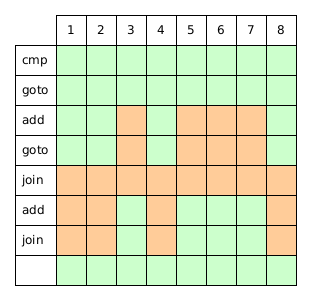
\includegraphics[scale=0.60]{Images/HW-goto-example.png}
  \caption{Схема исполнения представленного примера с векторным потоком
  управления}
  \label{fig:HW-goto-example}
\end{figure}

На рисунке ~\ref{fig:HW-goto-example} схематично изображено, как будет
происходить исполнение данного кода. Цифрами сверху обозначены номера линий
исполнения в SIMD-8 АЛУ, зеленым обозначены включенные линии, а оранжевым -
выключенные.

\section{Интерфейс между языковыми frontend'ами и векторным компилятором}
\label{sec:Interface}

Одним из языков, используемых для разработки программ исполняемых на
видеокартах, является ISPC. ISPC (Implicit SPMD Program Compiler) - язык программирования, являющийся
расширением С и реализующий концепцию SPMD. ISPC также, как и CM, является
языком с раздельным исходным кодом. Изначально целевой архитектурой для данного
языка была только архитектура x86 с векторными расширениями, но позже была
добавлена поддержка для ARM процессоров с расширениями Neon, а также
графических ускорителей Intel.

Программа на языке ISPC является SPMD программой и компилируется для векторов
заранее известной зафиксированной длины. В такой программе могут быть как общие,
так и свои для каждого запущенного потока данные. Общие для всех потоков данные
отмечают как uniform переменные, остальные по умолчанию считаются varying. Таким
образом, получается, что varying переменная по факту является каким-то элементом
вектора и может быть любым из них.

Ниже приведен пример функции на языке ISPC.

\begin{verbatim}
void simple(uniform float vin[],
            uniform float vout[],
            uniform int count) {
    foreach (index = 0 ... count) {
        float v = vin[index];
        if (v < 3.)
            v = v * v;
        else
            v = sqrt(v);
        vout[index] = v;
    }
}
\end{verbatim}

В ISPC нет ограничений на векторный поток управления в
стандартных конструкциях языка, и on реализуется через использование в качестве
условия varying переменной. Но при этом, так как ISPC является языком для
нескольких совершенно разных платформ с совершенно разной архитектурой, в данном
языке невозможно использование зависимых от платформы интринсиков. Вместо этого
ISPC маскирует результаты операций после условных переходов для векторного потока
управления. Безусловным преимуществом такого подхода является
кроссплатформенность достигаемая таким решением, но для архитектуры графических
ускорителей Intel такой подход не позволяет использовать всех векторных
возможностей потока управления аппаратуры.

В связи с этим был предложен интефейс для frontend'ов языков использующих
векторный backend графического компилятора Intel. Так как интерфейс должен
представлять собой конструкцию на промежуточном
представлении LLVM IR, который не поддерживает векторный поток управления,
неизбежно возникает необходимость сводить векторное условие к скалярному виду.
Перед условным переходом необходимо проверить справедливо ли условие хоть для
одного элемента и выполнять переход только в таком случае. Для наибольшей
кроссплатформенности для подобных проверок следует использовать стандартные
интринсики LLVM \texttt{@llvm.vector.reduce.and} и
\texttt{@llvm.vector.reduce.or}. Также для frontend'ов, имеющих только
архитектуру графических ускорителей Intel как
целевую, допускается использовать для редукции условий платформозависимые
интринсики \text{@llvm.genx.any} и \text{@llvm.genx.any}, являющиеся полными
аналогами прежде упомянутых. Для сохранения семантического смысла и
поддержки платформ, на которых нет развитой поддержки векторного потока
управления, необходимо маскировать условием побочные эффекты дуги перехода.

Как не трудно заметить данный подход будет абсолютно валиден для
скалярных архитектур, поддерживающих необходимые минимальные векторные
расширения. При этом в процессе оптимизаций компилятор не сможет сделать
трансформации меняющие смысл контекста, так как такая конструкция будет валидна
на всех этапах своего существования.

\section{Оптимизация}
\label{sec:Optimization}

Оптимизацией должен являться LLVM Pass из LLVM IR в LLVM IR в векторном
backend'е графического компилятора Intel. Для упрощения проектирования,
реализации и поддержки, оптимизация разделена на две части: анализ и
трансформацию.

Перед рассмотрением анализа и трансформации, проведем обзор возможных
конструкций, которые ожидаются на вход оптимизации.

Так как рассматривается только структурированный поток управления, то можно
рассматривать только два атомарных случая: векторный условный переход и
векторный цикл. На рисунках ~\ref{fig:if-else-simdcf-simple} и
~\ref{fig:loop-simdcf-simple} представлен граф потока управления для if-else и
цикла соответственно.
\begin{figure}
  \centering
  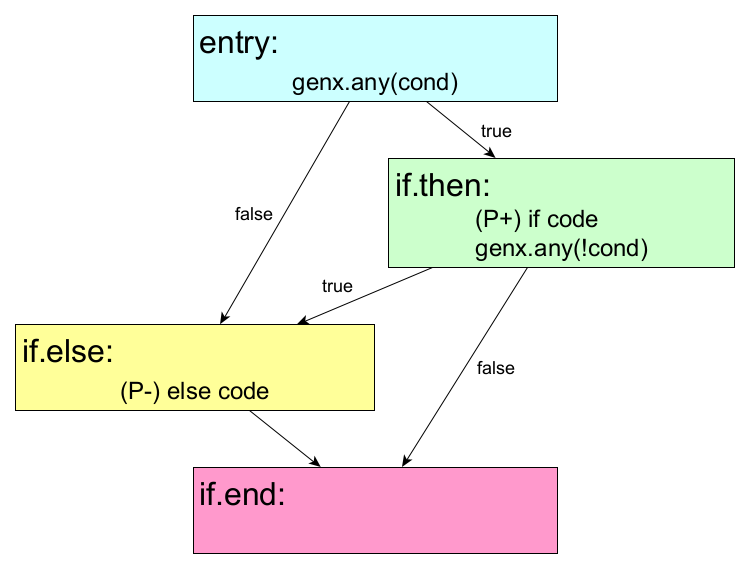
\includegraphics[scale=0.27]{Images/if-else-FE-colored.png}
  \caption{Схема потока управления для if-else}
  \label{fig:if-else-simdcf-simple}
\end{figure}
\begin{figure}
  \centering
  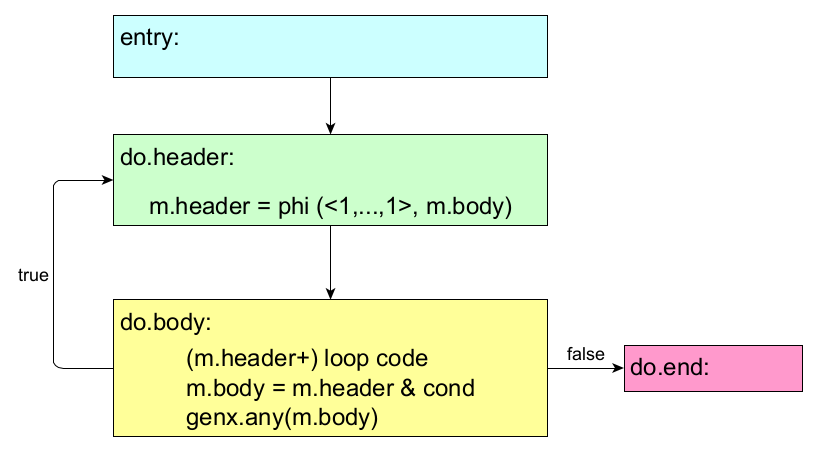
\includegraphics[scale=0.27]{Images/do-while-FE-colored.png}
  \caption{Схема потока управления для цикла}
  \label{fig:loop-simdcf-simple}
\end{figure}

В реальном коде может встречаться сложный поток управления, в котором базовые
паттерны могут являться элементами других базовых паттернов, образовывая
вложенные конструкции, например if-else вложенный в if-else (рисунок
~\ref{fig:nested-if-simdcf}) или цикл с вложенным if-else (рисунок
~\ref{fig:loop-nested-if-simdcf}).
\begin{figure}
  \centering
  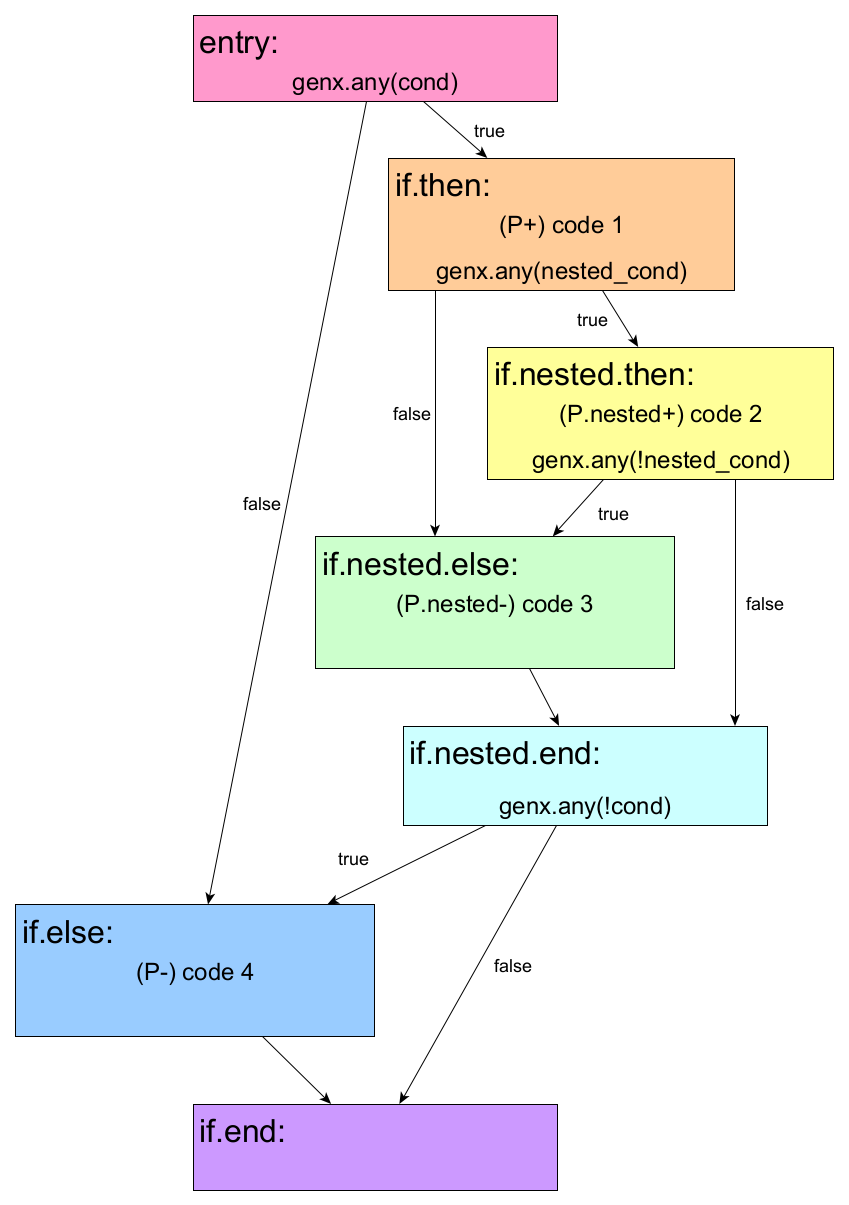
\includegraphics[scale=0.27]{Images/nested-if-FE-colored.png}
  \caption{Схема потока управления для случая if-else вложенного в if-else}
  \label{fig:nested-if-simdcf}
\end{figure}
\begin{figure}
  \centering
  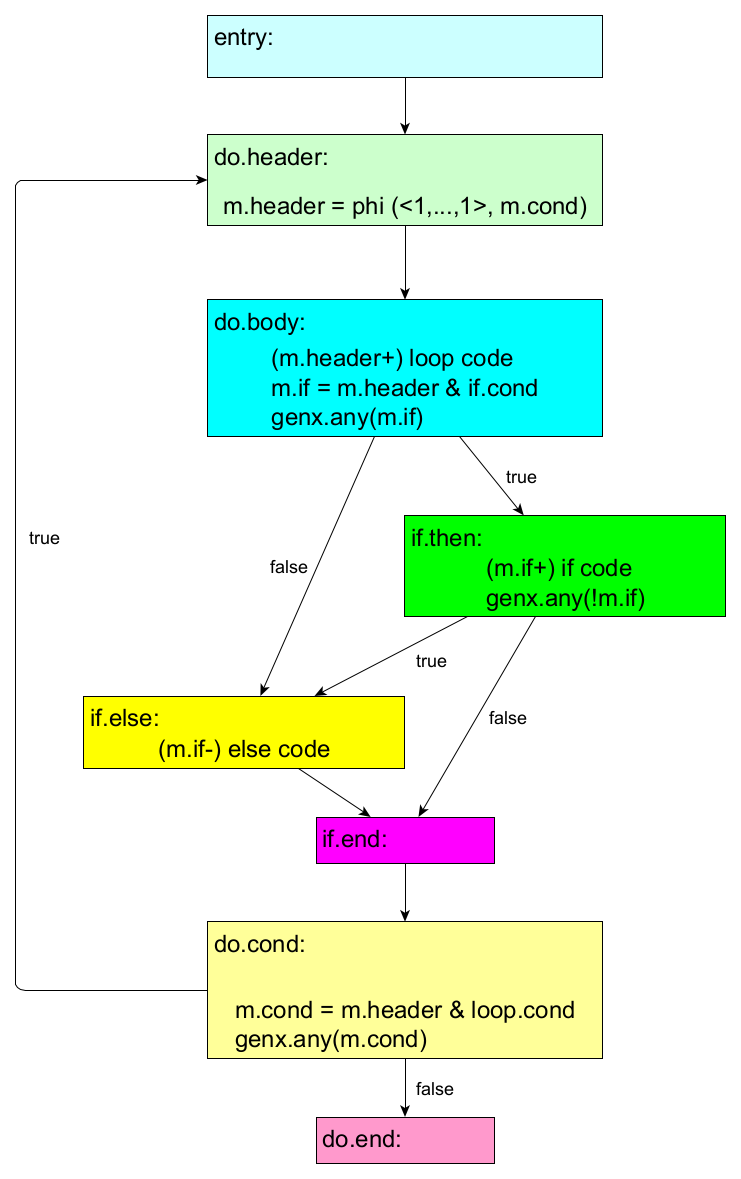
\includegraphics[scale=0.27]{Images/do-while-nested-if-FE-colored.png}
  \caption{Схема потока управления для случая if-else вложенного в цикл}
  \label{fig:loop-nested-if-simdcf}
\end{figure}

Можно выделить регионы, содержащие в себе одну конструкцию векторного потока
управления определенного уровня вложенности. Определим SIMD CF регион как
регион, содержащий в себе одну конструкцию предложенного ранее интерфейса самого
внешнего уровня вложенности, доступного для данного региона. Такой подход
позволит упростить анализ, позволяя сначала обнаруживать самые внешние SIMD CF
регионы, а после - вложенные. Тогда обобщенные SIMD CF регионы будут выглядеть
как на рисунках ~\ref{fig:generalized-if-simdcf} и ~\ref{fig:generalized-loop-simdcf}.
\begin{figure}
  \centering
  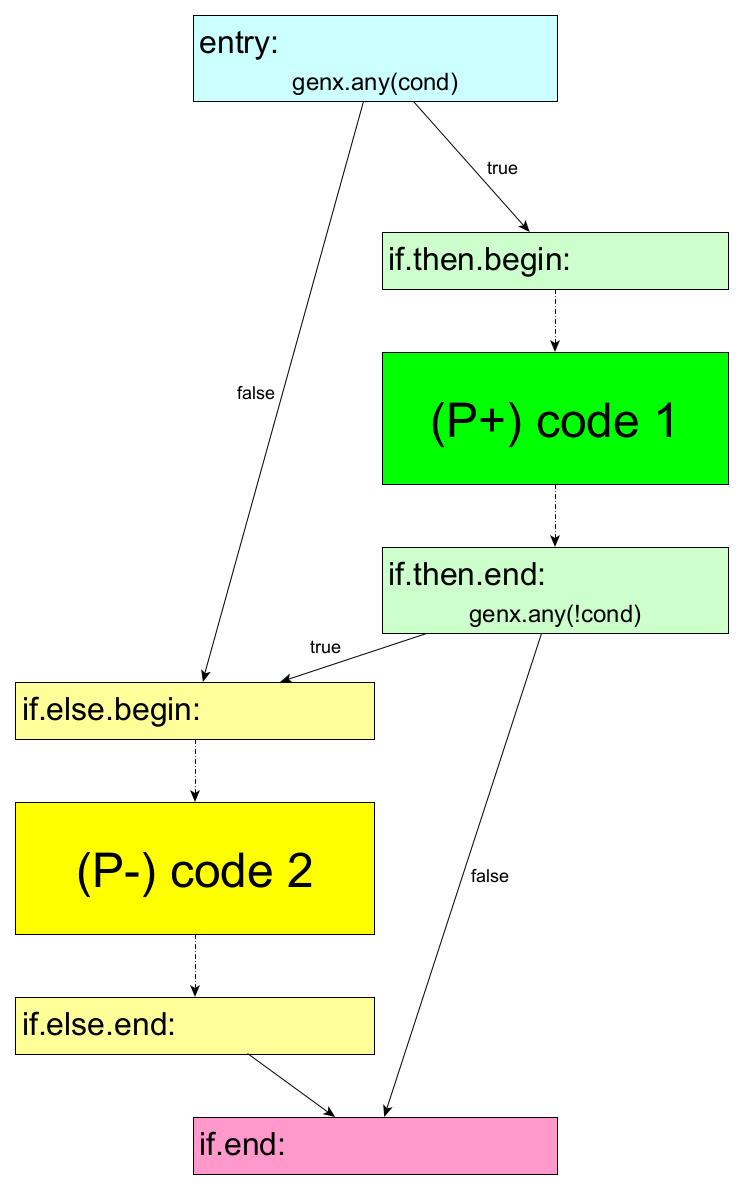
\includegraphics[scale=0.27]{Images/if-else-FE-generalized-colored.png}
  \caption{Схема if-else SIMD CF региона}
  \label{fig:generalized-if-simdcf}
\end{figure}
\begin{figure}
  \centering
  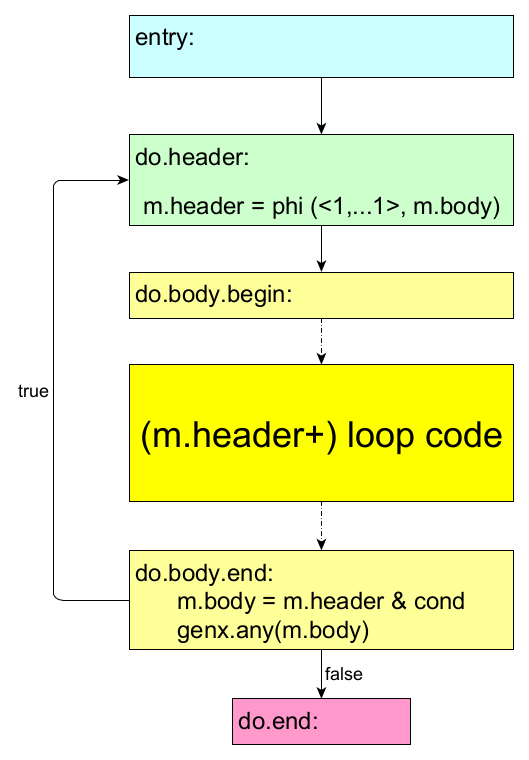
\includegraphics[scale=0.27]{Images/do-while-FE-generalized-colored.png}
  \caption{Схема if-else SIMD CF региона}
  \label{fig:generalized-loop-simdcf}
\end{figure}

После определения SIMD CF региона можно свести задачу поиска заранее оговоренных
конструкций к поиску SIMD CF регионов самого внешнего уровня вложенности, после
чего искать вложенные SIMD CF регионы.

Шаг 1. Поиск условного перехода, похожего на векторный поток управления. Для
каждого базового блока проверяется его терминатор. Если это инструкция условного
перехода, то проверяется его условие, в противном случае конструкция не является
SIMD CF регионом. Если условием является результат вызова одного из обозначенных
ранее интринсиков, то идет переход к шагу 2.

Шаг 2. Проверяется структура потока управления и происходит попытка сопоставить
его либо с SIMD CF if/else, либо с SIMD CF циклом. Если сопоставление с одним из
заданных паттернов невозможно, то конструкция не является SIMD CF регионом. В
противном случае происходит переход к шагу 3.

Шаг 3. Проверка маскирования побочных эффектов. Для каждой инструкции, у которой
есть побочные эффекты проводится проверка, является ли такая инструкция
маскирована и если она маскирована, то проверяется, совпадает ли маска для
данной инструкции с условием перехода в эту дугу. Для вложенных регионов
проверяется, является ли маска данного региона подмножеством маски внешнего
региона. Если проверка неудачная - данный регион не является SIMD CF регионом.

Дополнение к шагу 3 для цикла. Проверяются фи-узлы для индуктивностей и пересчет
маски для каждого цикла. Если проверка неудачная - данный регион не является
SIMD CF регионом. В противном случае идет переход к шагу 4.

Дополнение к шагу 3 для if-else. Если кроме if также имеется else, то происходит
проверка, являются ли маски if и else строго противоположны друг другу. Если
проверка неудачная - данный регион не является SIMD CF регионом. В противном
случае идет переход к шагу 4.

Шаг 4. Данный регион является SIMD CF регионом. Аналогично происходит поиск
вложенных SIMD CF регионов для данного региона.

В псевдокоде данный алгоритм будет выглядеть следующим образом:

\begin{verbatim}
procedure Find_SIMD_CF_Regions(Reg) returns set of SIMD_CF_Region
  Reg: Region
begin
  regions: set of SIMD_CF_Region
  bb: Basic_Block
  for each bb ∈ Reg do
    if Is_SIMD_CF_Branch(bb.terminator) then
      match: SIMD_CF_Region
      match := Match(bb)
      if match then
        if Verify(match) then
          regions ⋃= match
        fi
      fi
    fi
  od
  return regions
end

procedure Is_SIMD_CF_Branch(Term) return boolean
  Term: Instruction
begin
  cond: Instruction
  cond := Term.condition
  return cond ∈ {llvm.vector.reduce.and, llvm.vector.reduce.or}
end

procedure Match(BB) return SIMD_CF_Region
  BB: Basic_Block
begin
  if MatchIf(BB) then
    return SIMD_CF_If_Region(BB)
  elif MatchLoop(BB) then
    return SIMD_CF_Loop_Region(BB)
  else
    return nil
end

procedure MatchIf(Entry) return SIMD_CF_If_Region
  Entry: Basic_Block
begin
  subregions: set of SIMD_CF_Region
  has_else: boolean
  if_begin: Basic_Block
  if_end: Basic_Block
  else_begin: Basic_Block
  else_end: Basic_Block
  exit: Basic_Block
  if_begin := Entry.true_succ
  else_begin := Entry.false_succ
  pred: Basic_Block
  for each pred ∈ else_begin.preds do
    if pred ≠ Entry then
      if_end := pred
    fi
  od
  subregions ⋃= Find_SIMD_CF_Regions(Region(if_begin, if_end))
  if !if_end.terminator.conditional then
    has_else := false
    exit := else_begin
    return SIMD_CF_If_Region(Entry, exit, has_else, subregions)
  fi
  has_else := true
  exit := if_end.false_succ
  for each pred ∈ exit.preds do
    if pred ≠ if_end then
      else_end := pred
    fi
  od
  subregions ⋃= Find_SIMD_CF_Regions(Region(else_begin, else_end))
  return SIMD_CF_If_Region(Entry, exit, has_else, subregions)
end

procedure MatchLoop(BranchingBB) return SIMD_CF_Loop_Region
  BranchingBB: Basic_Block
begin
  loop: Loop
  loop := Get_Loop(BranchingBB)
  if !loop then
    return nil
  fi
  subregions ⋃= Find_SIMD_CF_Regions(Region(loop.entering, loop.exiting))
  return SIMD_CF_Loop_Region(loop, subregions)
end

procedure Verify(R) return boolean
  R: SIMD_CF_Region
begin
  inst: Instruction
  subreg: SIMD_CF_Region
  for each inst ∈ R do
    if inst.has_side_effects then
      if inst.mask ≠ R.mask then
        return false
      fi
    fi
  od
  for each subreg ∈ R.subregions do
    if !R.is_submask(subreg_mask) then
      return false
    fi
  od
  return true
end
\end{verbatim}

После сбора всей информации о SIMD CF регионах начинается их оптимизирующая
трансформация.

Для этого сначала рассмотрим текущую модель \texttt{goto}-\texttt{join} в
векторном backend'е графического компилятора Intel. Текущая модель для условных
переходов и циклов показана на рисунках ~\ref{fig:if-goto-join-BE} и
~\ref{fig:loop-goto-join-BE}.
\begin{figure}
  \centering
  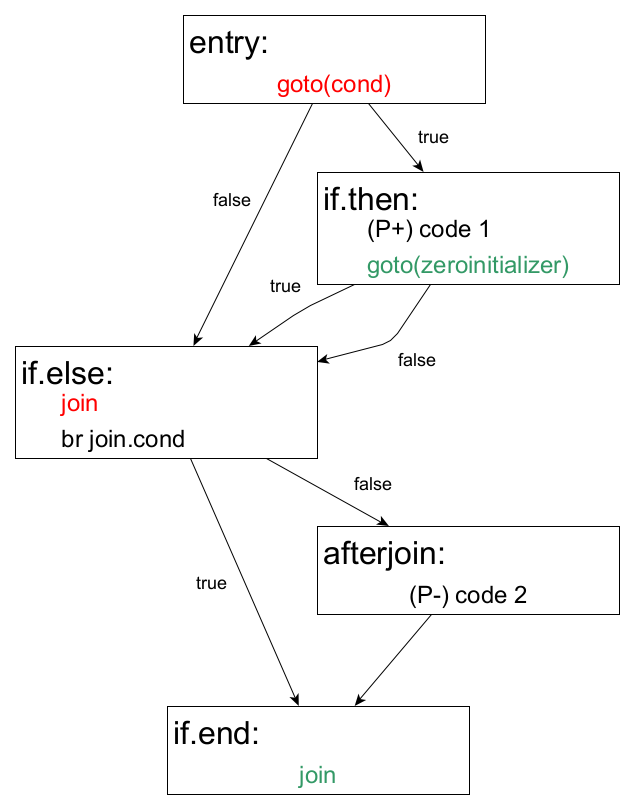
\includegraphics[scale=0.27]{Images/if-else-BE-current.png}
  \caption{\texttt{goto}-\texttt{join} cхема if-else в backend'е}
  \label{fig:if-goto-join-BE}
\end{figure}
\begin{figure}
  \centering
  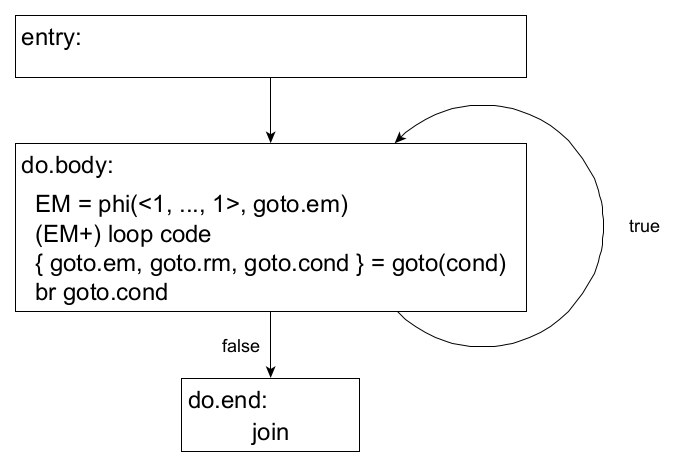
\includegraphics[scale=0.27]{Images/do-while-BE-current.png}
  \caption{\texttt{goto}-\texttt{join} cхема цикла в backend'е}
  \label{fig:loop-goto-join-BE}
\end{figure}

Для трансформирования разработанного интерфейса в уже имеющуюся модель
\texttt{goto}-\texttt{join}. Для этого надо заменить интринсик
\texttt{llvm.vector.reduce.and} или \texttt{llvm.vector.reduce.and} на
интринсик, соответствующий инструкции \texttt{goto} для вычисления условия
условного перехода, вставить соответствующий ему \texttt{join},
после чего убрать маскирование побочных эффектов.

Тогда мы получим следующие схемы для трансформации, представленные на рисунках
~\ref{fig:if-transform} и ~\ref{fig:loop-transform}.
\begin{figure}
  \centering
  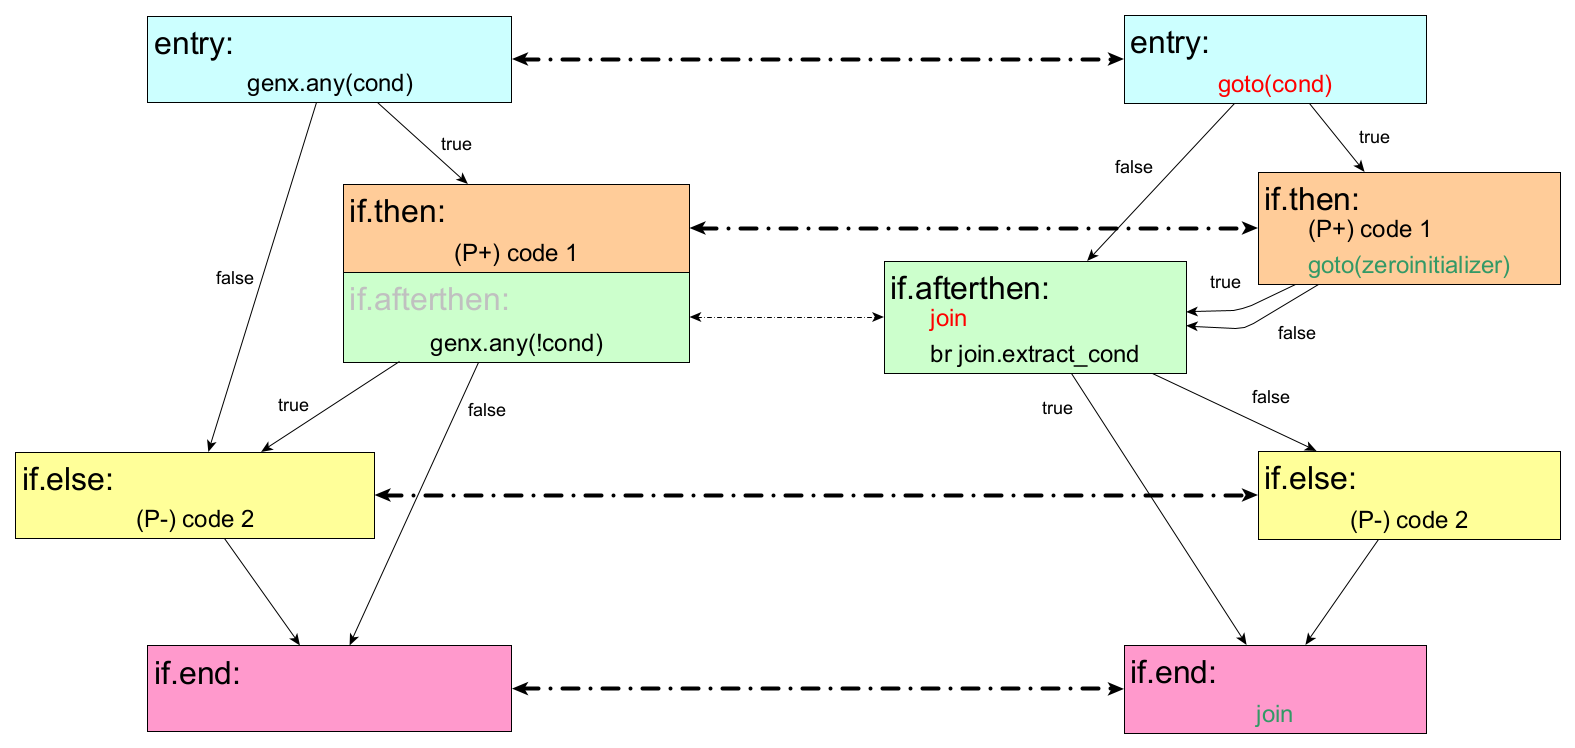
\includegraphics[width=0.5\textwidth]{Images/if-else-BE.png}
  \caption{Трансформация if-else}
  \label{fig:if-transform}
\end{figure}
\begin{figure}
  \centering
  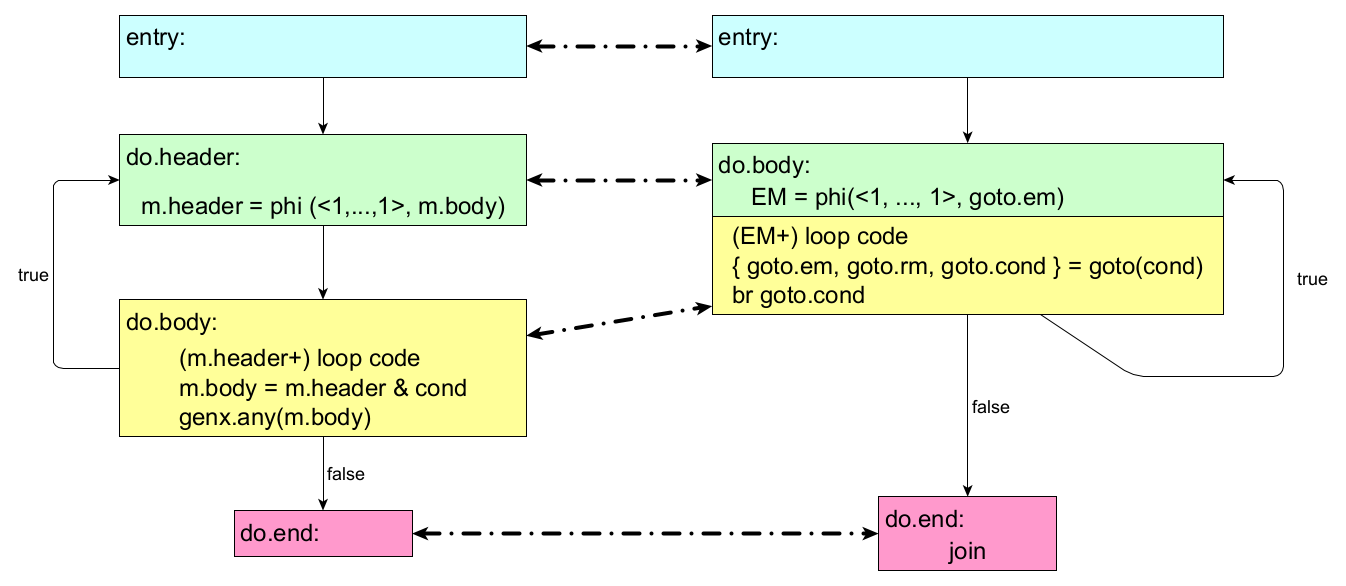
\includegraphics[width=0.5\textwidth]{Images/do-while-BE.png}
  \caption{Трансформация цикла}
  \label{fig:loop-transform}
\end{figure}

\section{Результаты}
\label{sec:conclusion-future}

%%----------------------------------------------------------------------------------%%
%% 								PAPER ACKNOWLEDGEMENT
%%----------------------------------------------------------------------------------%%
%\section*{Acknowledgement}
%The preferred spelling of the word ``acknowledgement'' in America is without 
%an ``e'' after the ``g''. Avoid the stilted expression ``one of us (R. B. 
%G.) thanks $\ldots$''. Instead, try ``R. B. G. thanks$\ldots$''. Put sponsor 
%acknowledgements in the unnumbered footnote on the first page.

%%----------------------------------------------------------------------------------%%
%% 							BIBLOGRAPHY (PAPER REFERENCES)
%%----------------------------------------------------------------------------------%%
\bibliographystyle{IEEEtran}
\bibliography{IEEEabrv,IEEEReferences}
%%----------------------------------------------------------------------------------%%
\end{document}
